\section{Definitions}
\label{sec:definitions}

In this Section, a series of terms, which are used throughout this Thesis, is introduced.

\subsection{Privacy terms}
\label{sec:def_privacy_terms}

The expression \textit{`privacy terms'} is usually associated with the notice that personal data handling entities use to disclose how they collect, use, store, secure, and share personal data (\ref{sec:def_personal_data}).
% In this Thesis, it has a broader meaning -- the term ``privacy term'' will be used to refer to the information that needs to be modelled in data requests by entities seeking access to personal data, in user policies where data subjects express their preferences and requirements when it comes to the processing of their own data and in data access agreements where the conditions for the access to personal data are recorded.
In this Thesis, it has a broader meaning -- the expression \textit{`privacy term'} will be used to refer to the information that needs to be modelled to represent concepts related to the preferences and rights of data subjects and to the policies (\ref{sec:def_policies}) and obligations of data controllers regarding privacy and personal data protection~\citep{esteves_challenges_2021}.
Examples of privacy terms are the \textit{purpose} for processing personal data, the \textit{processing operation} itself, the \textit{legal basis} used by the data controller to justify the processing, or the \textit{right to data portability}.

\subsection{Policies}
\label{sec:def_policies}

Policies are documents that describe conditions for access and usage of content. Such policies can be expressed as permissions, prohibitions, or obligations and include constraints, i.e., conditions that refine the policy rules~\citep{iannella_odrl_2018}.
In this Thesis, the focus will be on the design of policies to determine access to personal data assets stored in decentralised data systems. Examples of these policies are \textit{user preferences and requirements}, \textit{applications privacy policies} and \textit{data requests} or \textit{data access agreements} regarding data handling practices over personal data stored or shared through personal datastores (\ref{sec:def_pds}).

\subsection{Access control}
\label{sec:def_access_control}

The term \textit{`access control'} refers to the model used to guide the process of access to resources. To do so, access control rules can be defined through a policy language (\ref{sec:def_policies}) with specific syntax and semantics, which are the base of a policy enforcement mechanism~\citep{cuenca_grau_access_2017}. Moreover, both authentication and authorisation mechanisms (processes related to identity verification and rule-based access control enforcement, respectively) are involved in the process of granting or denying access to resources. In simple terms, an access control policy involves three aspects: (i) the entity requesting/being requested access, (ii) the requested resource(s), and (iii) the access rules, i.e., permissions and prohibitions on particular access modes.

\subsection{Legislation on data protection}
\label{sec:def_data_protection_law}

Before data protection was considered a fundamental right, the right to privacy emerged in 1948 through the Universal Declaration of Human Rights (UDHR) under Article 12, which stated that \textit{``No one shall be subjected to arbitrary interference with his privacy, family, home or correspondence [...]''}~\citep{united_nations_general_assembly_universal_1948}, and through the European Convention on Human Rights (ECHR) under Article 8 as \textit{``Everyone has the right to respect for his private and family life, his home and his correspondence''}~\citep{council_of_europe_european_1950}.

The first and only legally binding international instrument in the field of data protection, Convention 108~\citep{council_of_europe_convention_1981}, was created by the Council of Europe in 1981 and has been improved throughout the years to deal with automatic processing, supervisory authorities, and transborder data flows.
Following in these footsteps, the Charter of Fundamental Rights of the EU~\citeyearpar{noauthor_charter_2000}, under Article 8, acknowledged that \textit{``Everyone has the right to the protection of personal data concerning him or her''} and that \textit{``Such data must be processed fairly for specified purposes and on the basis of the consent of the person concerned or some other legitimate basis laid down by law''}, in addition to the right to privacy laid down in Article 7, and in 1995 the first EU law on data protection, the Data Protection Directive~\citeyearpar{noauthor_directive_1995}, was launched.

Further legislation was enforced in 2018 to adapt the EU law on data protection to the intensive usage of digital personal data (\ref{sec:def_personal_data}) by new technological developments in the form of the GDPR~\citeyearpar{noauthor_regulation_2016}.
In the same package, the EU launched a similar piece of legislation for the processing of personal data by state authorities for law enforcement purposes, i.e., preventing, investigating, detecting, and prosecuting criminal offences or executing criminal penalties, the Directive 2017/680~\citeyearpar{noauthor_directive_2016}.

This Thesis focuses on the requirements brought by the GDPR (\ref{sec:def_gdpr}) and also resorts to the opinions and guidelines adopted by the Article 29 Working Party, EDPB and EDPS, as well as case law and other legal literature~\citep{european_union_agency_for_fundamental_rights_and_council_of_europe_handbook_2018}.

\subsubsection{GDPR}
\label{sec:def_gdpr}

GDPR~\citeyearpar{noauthor_regulation_2016} is the landmark legislation on data protection in Europe and its effects have been felt throughout the globe, with similar pieces of regulation being discussed and adopted in American, African, and Asian countries~\citep{bradford_brussels_2019}. It established the following principles related to the processing of personal data:
\begin{enumerate}
    \item [(i)] it should be processed in a legal, fair, and transparent manner (Article 5.1(a) on \textit{`lawfulness, fairness and transparency'}).
    \item [(ii)] the processing should be limited to the purpose specified by the data subject (Article 5.1(b) on \textit{`purpose limitation'}).
    \item [(iii)] it should include only the minimum data relevant to the purpose for which it is being processed (Article 5.1(c) on \textit{`data minimisation'}).
    \item [(iv)] the data should be accurate and possible to be corrected when necessary (Article 5.1(d) on \textit{`accuracy'}).
    \item [(v)] it should be kept only as long as it is necessary (Article 5.1(e) on \textit{`storage limitation'}).
    \item [(vi)] adequate technical and organisational measures for the security of the personal data should be ensured (Article 5.1(f) on \textit{`integrity and confidentiality'}).
    \item [(vii)] data controllers should have accountability mechanisms to demonstrate compliance with these principles (Article 5.2 on \textit{`accountability'}).
\end{enumerate}

Moreover, while analysing Chapters III and IV (\textit{`Rights of the data subject'}\footnote{\url{https://gdpr-info.eu/chapter-3/} (accessed on 15 March 2024)} and \textit{`Controller and processor'}\footnote{\url{https://gdpr-info.eu/chapter-4/} (accessed on 15 March 2024)}, respectively) of the GDPR, a set of information flows between data-related entities, i.e., data subjects, data controllers, processors and data protection officers, recipients, or supervisory authorities, can be identified.
In this context, an information flow refers to the information that has to be shared between entities so that a right or obligation can be exercised or fulfilled and GDPR's principles of lawfulness, fairness, and transparency can be respected.
For instance, if a data subject wishes to exercise its \textit{`right to erasure'}, apart from raising such a request, there is the need to represent information related to the grounds on which the request is based, and the data controller needs to forward this request to other controllers which are processing the same personal data.
Figure \ref{fig:gdpr_information_flows} shows a diagram of such information flows.

While the focus of this Thesis relies on the fulfilment of data subjects' rights, it is important to notice as well that the GDPR also contains other provisions, including requirements on transfers of personal data to third countries or international organisations, or on the activities of data protection supervisory authorities.

\begin{landscape}
\begin{figure}
    \centering
    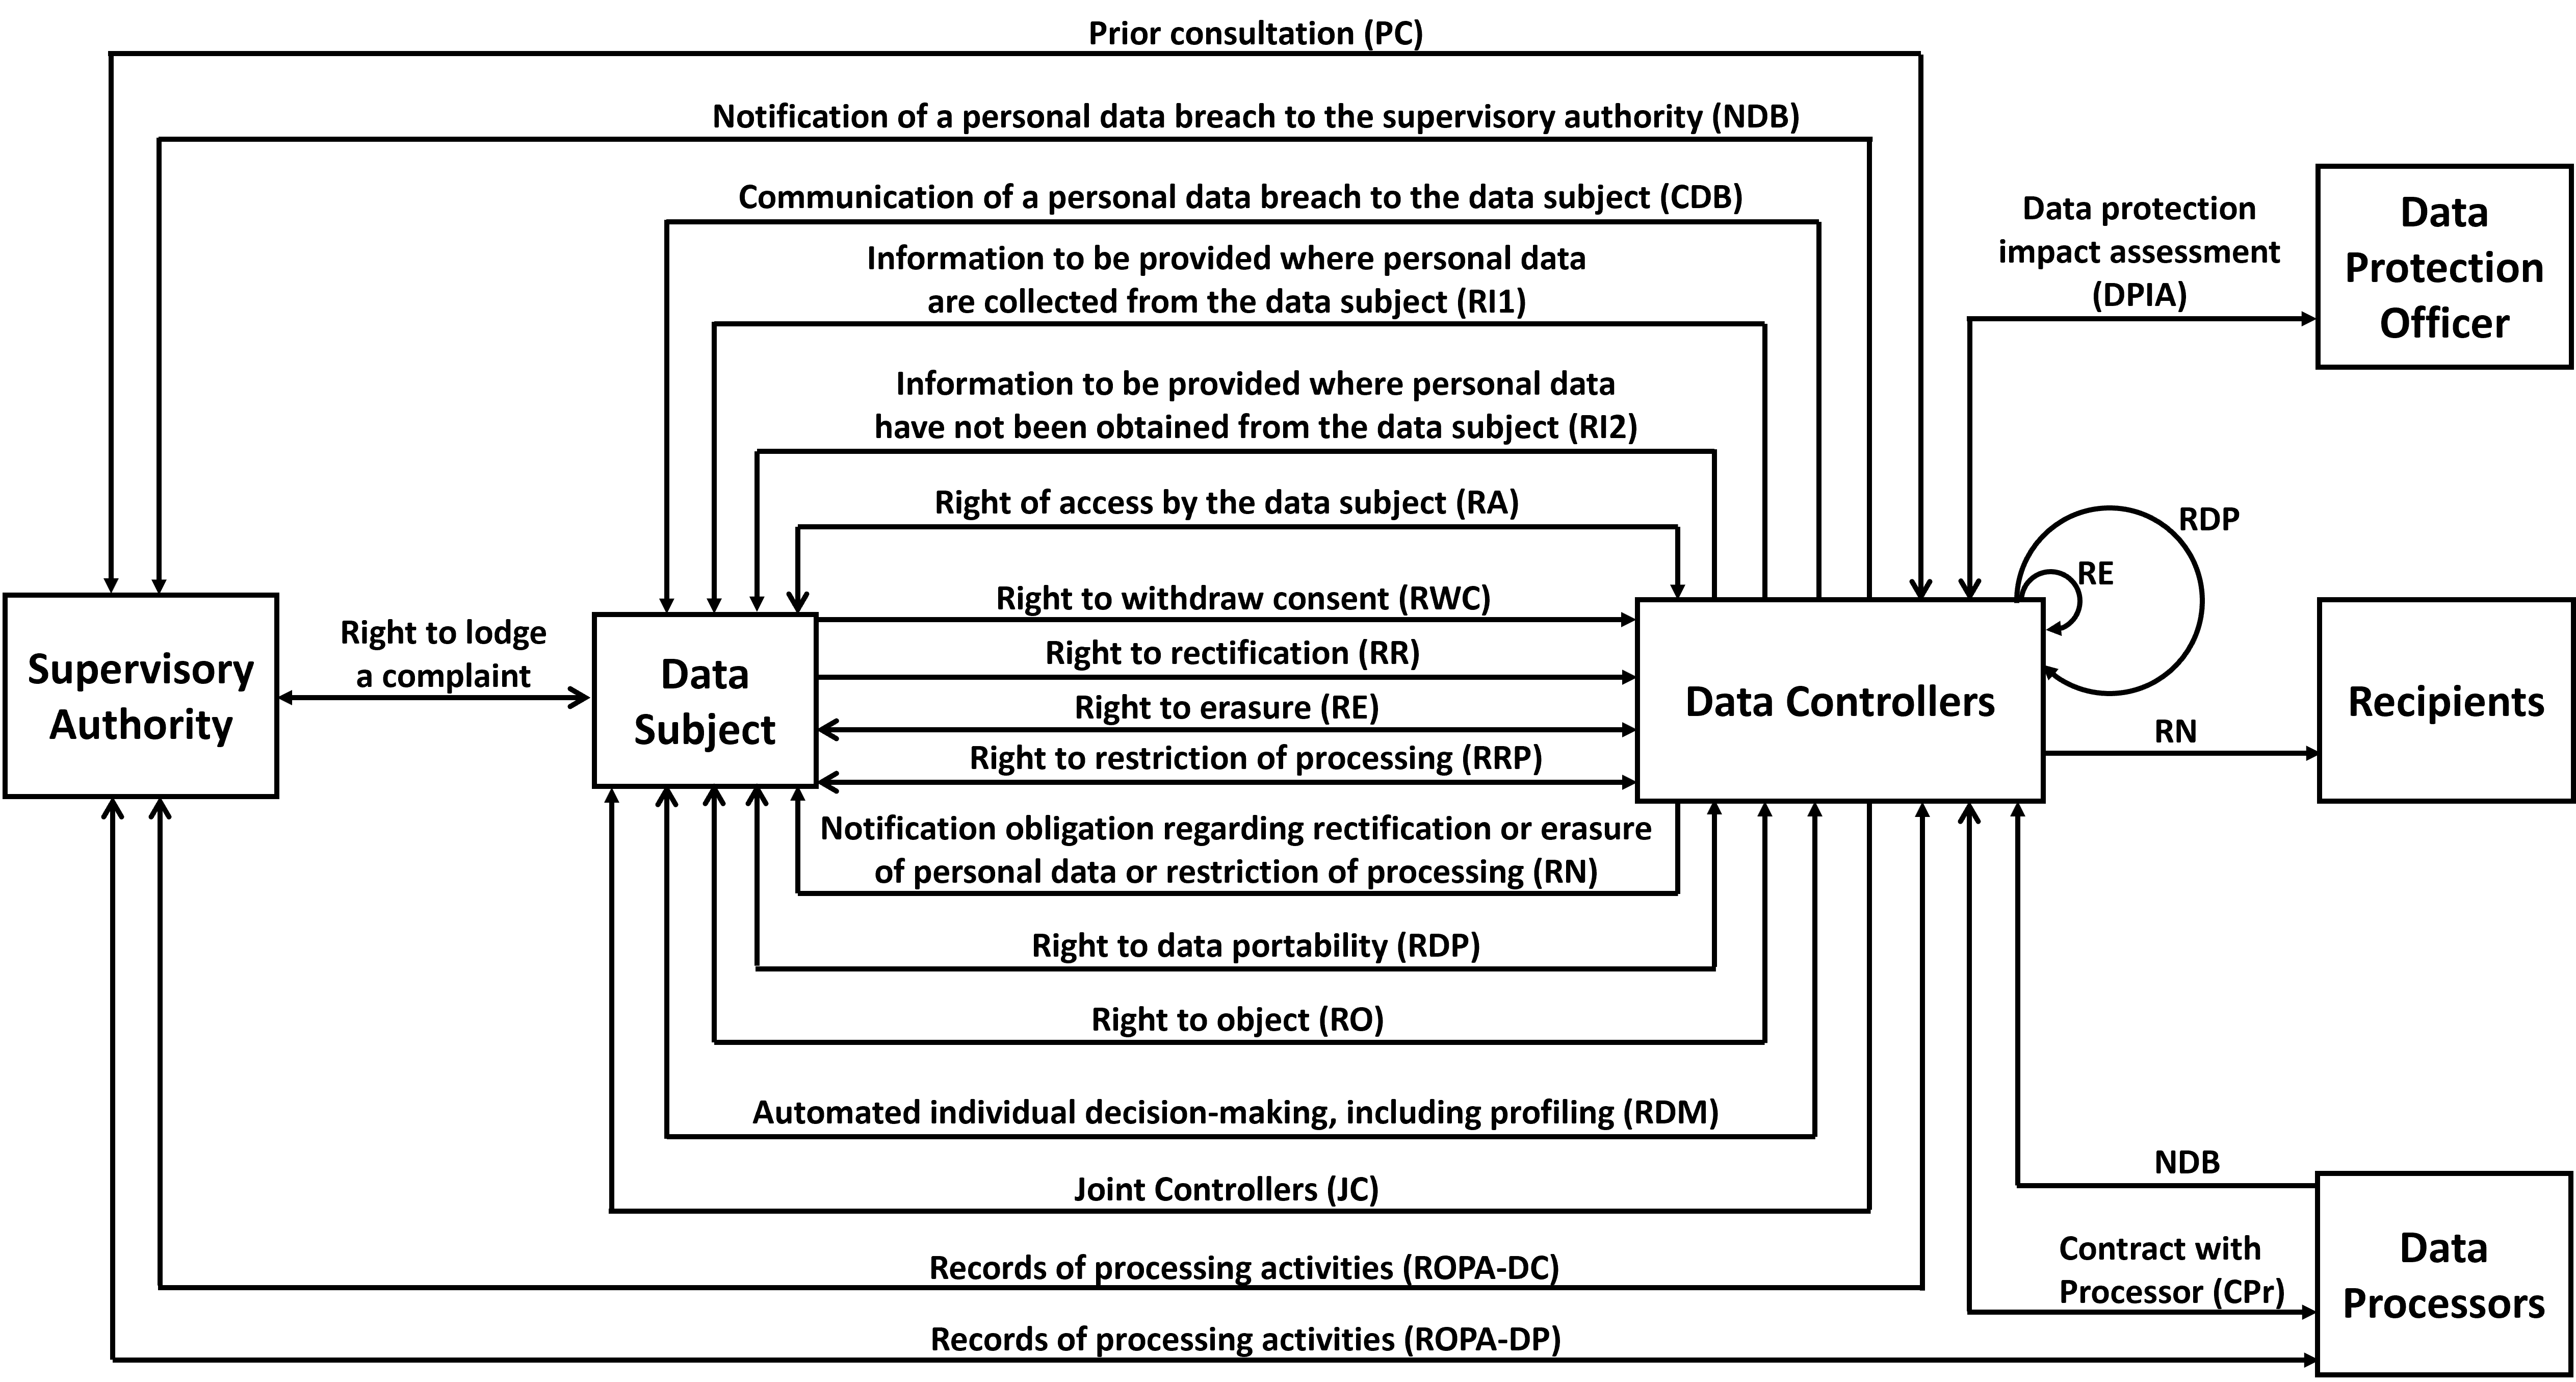
\includegraphics[width=\linewidth]{figures/chapter-1/information flow diagram.png}
    \caption[GDPR's rights and obligations as information flows.]{GDPR's rights and obligations as information flows. The bidirectional arrows represent a right or obligation in which a request for information and respective response is expected (the open arrowhead, \ding{220}, represents the entity waiting for the response and the closed arrowhead, \ding{225}, the entity being requested). In contrast, the unidirectional arrows represent only a request or notification and no reply is expected (with the closed arrowhead, \ding{225}, representing the entity being requested or notified), adapted from~\cite{esteves_analysis_2022}.}
    \label{fig:gdpr_information_flows}
\end{figure}
\end{landscape}

\subsection{Personal data}
\label{sec:def_personal_data}

GDPR's Article 4.1~\citeyearpar{noauthor_regulation_2016} defines `personal data' as \textit{``any information relating to an identified or identifiable natural person''} such as \textit{``a name, an identification number, location data, an online identifier or to one or more factors specific to the physical, physiological, genetic, mental, economic, cultural or social identity of that natural person''}.
This Thesis relies on GDPR's definition of personal data and special categories of personal data.
In addition, it is also acknowledged that there are categories of data that are sensitive, even though they are not considered `special' under GDPR's Article 9.1, which might require additional consideration and/or protection, e.g., location data has the potential to reveal religious beliefs, sexual orientation or political opinions\footnote{DPV models \url{https://w3id.org/dpv\#SensitivePersonalData} as a subtype of \url{https://w3id.org/dpv\#PersonalData} and \url{https://w3id.org/dpv\#SpecialCategoryPersonalData} as a subtype of \url{https://w3id.org/dpv\#SensitivePersonalData}}.

Table \ref{tab:data_sensitivity}, derived from the analysis of~\cite{rumbold_what_2018}, illustrates data sensitivity for particular subcategories of data. For each data type, sensitivity is assessed from 0 to 10, i.e., from low to high sensitivity, and the relative frequency of falling into that particular sensitivity value, on a scale of 1 to 4, is also presented. For instance, data related to objects has a sensitivity of 0 and a frequency of 4 as it can not be used to identify a person, while occupation data would not be frequently classified as being highly sensitive, as demonstrated by the frequency value of 1 to the sensitivity value of 10.
In addition, data sensitivity assessment is highly contextual, as shown through the fact that the same data category can have a spectrum of sensitivity, e.g., anonymised data can have a low/high sensitivity if the risk of re-identification is very low/high, respectively. 
This evaluation of data sensitivity is also well aligned with GDPR's special categories of personal data, as can be seen through the last column of the table, where these special categories are identified and, indeed, the most sensitive are presented in Article 9, with the exception of social class data.

\begin{table}
\caption[Data sensitivity chart derived from~\cite{rumbold_what_2018}.]{Data sensitivity chart derived from~\cite{rumbold_what_2018}. GDPR's special categories of personal data are identified in the \textbf{GDPR} column.}
\label{tab:data_sensitivity}
\scriptsize
\begin{tabular}{|c|c||l|l|c|c|c|c|c|c|l|l|l||l|}
\multicolumn{2}{c}{} & \multicolumn{11}{c}{\textbf{DATA SENSITIVITY}} & \multicolumn{1}{c}{} \\
\hline
\multicolumn{2}{|c||}{\textbf{DATA TYPE}}                                                                                                                                                                                                                   & \multicolumn{1}{r|}{\cellcolor[HTML]{9A0000}{\color[HTML]{FFFFFF} 10}}         & \multicolumn{1}{r|}{\cellcolor[HTML]{CB0000}{\color[HTML]{FFFFFF} 9}}          & \multicolumn{1}{r|}{\cellcolor[HTML]{F56B00}{\color[HTML]{FFFFFF} 8}} & \multicolumn{1}{r|}{\cellcolor[HTML]{F8A102}7} & \multicolumn{1}{r|}{\cellcolor[HTML]{FFCB2F}6} & \multicolumn{1}{r|}{\cellcolor[HTML]{FFFE65}5} & \multicolumn{1}{r|}{\cellcolor[HTML]{D9EF8B}4} & \multicolumn{1}{r|}{\cellcolor[HTML]{A6D96A}{\color[HTML]{FFFFFF} 3}} & \multicolumn{1}{r|}{\cellcolor[HTML]{66BD63}{\color[HTML]{FFFFFF} 2}}          & \multicolumn{1}{r|}{\cellcolor[HTML]{1A9850}{\color[HTML]{FFFFFF} 1}}          & \multicolumn{1}{r||}{\cellcolor[HTML]{036400}{\color[HTML]{FFFFFF} 0}}          & \textbf{GDPR}   \\ \hline\hline
\multicolumn{1}{|c|}{}                                                                                                                                   & Relating to objects                                                                            &                                                                                &                                                                                & \multicolumn{1}{l|}{}                                                 & \multicolumn{1}{l|}{}                          & \multicolumn{1}{l|}{}                          & \multicolumn{1}{l|}{}                          & \multicolumn{1}{l|}{}                          & \multicolumn{1}{l|}{}                                                 &                                                                                &                                                                                & \multicolumn{1}{c||}{\cellcolor[HTML]{036400}{\color[HTML]{FFFFFF} \textbf{4}}} &                 \\ \cline{2-14}
\multicolumn{1}{|c|}{\multirow{-2}{*}{\textbf{\begin{tabular}[c]{@{}c@{}}Non-personal\\ data\end{tabular}}}}                                             & \begin{tabular}[c]{@{}c@{}}Anonymised data\\ related to persons\end{tabular}                   &                                                                                &                                                                                & \cellcolor[HTML]{F56B00}{\color[HTML]{FFFFFF} \textbf{1}}             & \cellcolor[HTML]{F8A102}\textbf{1}             & \cellcolor[HTML]{FFCB2F}\textbf{1}             & \cellcolor[HTML]{FFFE65}\textbf{1}             & \cellcolor[HTML]{D9EF8B}\textbf{2}             & \cellcolor[HTML]{A6D96A}{\color[HTML]{FFFFFF} \textbf{3}}             & \multicolumn{1}{c|}{\cellcolor[HTML]{66BD63}{\color[HTML]{FFFFFF} \textbf{3}}} & \multicolumn{1}{c|}{\cellcolor[HTML]{1A9850}{\color[HTML]{FFFFFF} \textbf{4}}} & \multicolumn{1}{c||}{\cellcolor[HTML]{036400}{\color[HTML]{FFFFFF} \textbf{3}}} &                 \\ \hline\hline
\multicolumn{1}{|c|}{}                                                                                                                                   & Opinions                                                                                       &                                                                                &                                                                                & \multicolumn{1}{l|}{}                                                 & \cellcolor[HTML]{F8A102}\textbf{3}             & \cellcolor[HTML]{FFCB2F}\textbf{3}             & \cellcolor[HTML]{FFFE65}\textbf{3}             & \cellcolor[HTML]{D9EF8B}\textbf{3}             & \cellcolor[HTML]{A6D96A}{\color[HTML]{FFFFFF} \textbf{3}}             & \multicolumn{1}{c|}{\cellcolor[HTML]{66BD63}{\color[HTML]{FFFFFF} \textbf{3}}} & \multicolumn{1}{c|}{\cellcolor[HTML]{1A9850}{\color[HTML]{FFFFFF} \textbf{3}}} &                                                                                &                 \\ \cline{2-14}
\multicolumn{1}{|c|}{}                                                                                                                                   & Purchasing habits                                                                              &                                                                                &                                                                                & \cellcolor[HTML]{F56B00}{\color[HTML]{FFFFFF} \textbf{1}}             & \cellcolor[HTML]{F8A102}\textbf{2}             & \cellcolor[HTML]{FFCB2F}\textbf{3}             & \cellcolor[HTML]{FFFE65}\textbf{3}             & \cellcolor[HTML]{D9EF8B}\textbf{3}             & \cellcolor[HTML]{A6D96A}{\color[HTML]{FFFFFF} \textbf{3}}             & \multicolumn{1}{c|}{\cellcolor[HTML]{66BD63}{\color[HTML]{FFFFFF} \textbf{3}}} & \multicolumn{1}{c|}{\cellcolor[HTML]{1A9850}{\color[HTML]{FFFFFF} \textbf{3}}} &                                                                                &                 \\ \cline{2-14}
\multicolumn{1}{|c|}{}                                                                                                                                   & Sex                                                                                            &                                                                                &                                                                                & \multicolumn{1}{l|}{}                                                 & \multicolumn{1}{l|}{}                          & \multicolumn{1}{l|}{}                          & \multicolumn{1}{l|}{}                          & \cellcolor[HTML]{D9EF8B}\textbf{3}             & \cellcolor[HTML]{A6D96A}{\color[HTML]{FFFFFF} \textbf{3}}             & \multicolumn{1}{c|}{\cellcolor[HTML]{66BD63}{\color[HTML]{FFFFFF} \textbf{3}}} &                                                                                &                                                                                &                 \\ \cline{2-14}
\multicolumn{1}{|c|}{}                                                                                                                                   & Age                                                                                            &                                                                                &                                                                                & \multicolumn{1}{l|}{}                                                 & \cellcolor[HTML]{F8A102}\textbf{3}             & \cellcolor[HTML]{FFCB2F}\textbf{3}             & \cellcolor[HTML]{FFFE65}\textbf{3}             & \cellcolor[HTML]{D9EF8B}\textbf{3}             & \cellcolor[HTML]{A6D96A}{\color[HTML]{FFFFFF} \textbf{3}}             &                                                                                &                                                                                &                                                                                &                 \\ \cline{2-14}
\multicolumn{1}{|c|}{}                                                                                                                                   & Income                                                                                         &                                                                                &                                                                                & \cellcolor[HTML]{F56B00}{\color[HTML]{FFFFFF} \textbf{2}}             & \cellcolor[HTML]{F8A102}\textbf{3}             & \cellcolor[HTML]{FFCB2F}\textbf{3}             & \cellcolor[HTML]{FFFE65}\textbf{3}             & \cellcolor[HTML]{D9EF8B}\textbf{3}             & \cellcolor[HTML]{A6D96A}{\color[HTML]{FFFFFF} \textbf{3}}             &                                                                                &                                                                                &                                                                                &                 \\ \cline{2-14}
\multicolumn{1}{|c|}{}                                                                                                                                   & Location                                                                                       &                                                                                & \multicolumn{1}{c|}{\cellcolor[HTML]{CB0000}{\color[HTML]{FFFFFF} \textbf{1}}} & \cellcolor[HTML]{F56B00}{\color[HTML]{FFFFFF} \textbf{2}}             & \cellcolor[HTML]{F8A102}\textbf{3}             & \cellcolor[HTML]{FFCB2F}\textbf{3}             & \cellcolor[HTML]{FFFE65}\textbf{3}             & \cellcolor[HTML]{D9EF8B}\textbf{3}             & \cellcolor[HTML]{A6D96A}{\color[HTML]{FFFFFF} \textbf{3}}             &                                                                                &                                                                                &                                                                                &                 \\ \cline{2-14}
\multicolumn{1}{|c|}{}                                                                                                                                   & \begin{tabular}[c]{@{}c@{}}Lifestyle or\\ wellness data\end{tabular}                           &                                                                                & \multicolumn{1}{c|}{\cellcolor[HTML]{CB0000}{\color[HTML]{FFFFFF} \textbf{3}}} & \cellcolor[HTML]{F56B00}{\color[HTML]{FFFFFF} \textbf{3}}             & \cellcolor[HTML]{F8A102}\textbf{3}             & \cellcolor[HTML]{FFCB2F}\textbf{3}             & \cellcolor[HTML]{FFFE65}\textbf{3}             & \cellcolor[HTML]{D9EF8B}\textbf{3}             & \cellcolor[HTML]{A6D96A}{\color[HTML]{FFFFFF} \textbf{3}}             &                                                                                &                                                                                &                                                                                &                 \\ \cline{2-14}
\multicolumn{1}{|c|}{}                                                                                                                                   & Occupation                                                                                     & \multicolumn{1}{c|}{\cellcolor[HTML]{9A0000}{\color[HTML]{FFFFFF} \textbf{1}}} & \multicolumn{1}{c|}{\cellcolor[HTML]{CB0000}{\color[HTML]{FFFFFF} \textbf{2}}} & \cellcolor[HTML]{F56B00}{\color[HTML]{FFFFFF} \textbf{3}}             & \cellcolor[HTML]{F8A102}\textbf{3}             & \cellcolor[HTML]{FFCB2F}\textbf{3}             & \cellcolor[HTML]{FFFE65}\textbf{3}             & \cellcolor[HTML]{D9EF8B}\textbf{3}             & \cellcolor[HTML]{A6D96A}{\color[HTML]{FFFFFF} \textbf{3}}             &                                                                                &                                                                                &                                                                                &                 \\ \cline{2-14}
\multicolumn{1}{|c|}{}                                                                                                                                   & Address                                                                                        &                                                                                &                                                                                & \cellcolor[HTML]{F56B00}{\color[HTML]{FFFFFF} \textbf{2}}             & \cellcolor[HTML]{F8A102}\textbf{3}             & \cellcolor[HTML]{FFCB2F}\textbf{3}             & \cellcolor[HTML]{FFFE65}\textbf{3}             & \cellcolor[HTML]{D9EF8B}\textbf{3}             & \multicolumn{1}{l|}{}                                                 &                                                                                &                                                                                &                                                                                &                 \\ \cline{2-14}
\multicolumn{1}{|c|}{}                                                                                                                                   & Race                                                                                           &                                                                                &                                                                                & \cellcolor[HTML]{F56B00}{\color[HTML]{FFFFFF} \textbf{3}}             & \cellcolor[HTML]{F8A102}\textbf{3}             & \cellcolor[HTML]{FFCB2F}\textbf{3}             & \cellcolor[HTML]{FFFE65}\textbf{3}             & \cellcolor[HTML]{D9EF8B}\textbf{3}             & \multicolumn{1}{l|}{}                                                 &                                                                                &                                                                                &                                                                                & \textbf{Art. 9} \\ \cline{2-14}
\multicolumn{1}{|c|}{}                                 & Ethnic group                                                                                   &                                                                                &                                                                                & \cellcolor[HTML]{F56B00}{\color[HTML]{FFFFFF} \textbf{3}}             & \cellcolor[HTML]{F8A102}\textbf{3}             & \cellcolor[HTML]{FFCB2F}\textbf{3}             & \cellcolor[HTML]{FFFE65}\textbf{3}             & \cellcolor[HTML]{D9EF8B}\textbf{3}             & \multicolumn{1}{l|}{}                                                 &                                                                                &                                                                                &                                                                                & \textbf{Art. 9} \\ \cline{2-14}
\multicolumn{1}{|c|}{}                                                                                                                                   & \begin{tabular}[c]{@{}c@{}}Religious or\\ political beliefs\end{tabular}                       &                                                                                &                                                                                & \cellcolor[HTML]{F56B00}{\color[HTML]{FFFFFF} \textbf{3}}             & \cellcolor[HTML]{F8A102}\textbf{3}             & \cellcolor[HTML]{FFCB2F}\textbf{3}             & \cellcolor[HTML]{FFFE65}\textbf{3}             & \cellcolor[HTML]{D9EF8B}\textbf{3}             & \multicolumn{1}{l|}{}                                                 &                                                                                &                                                                                &                                                                                & \textbf{Art. 9} \\ \cline{2-14}
\multicolumn{1}{|c|}{}                                                                                                                                   & Sexual orientation                                                                             &                                                                                &                                                                                & \cellcolor[HTML]{F56B00}{\color[HTML]{FFFFFF} \textbf{3}}             & \cellcolor[HTML]{F8A102}\textbf{3}             & \cellcolor[HTML]{FFCB2F}\textbf{3}             & \cellcolor[HTML]{FFFE65}\textbf{3}             & \cellcolor[HTML]{D9EF8B}\textbf{3}             & \multicolumn{1}{l|}{}                                                 &                                                                                &                                                                                &                                                                                & \textbf{Art. 9} \\ \cline{2-14}
\multicolumn{1}{|c|}{}                                                                                                                                   & Pregnancy                                                                                      &                                                                                & \multicolumn{1}{c|}{\cellcolor[HTML]{CB0000}{\color[HTML]{FFFFFF} \textbf{3}}} & \cellcolor[HTML]{F56B00}{\color[HTML]{FFFFFF} \textbf{3}}             & \cellcolor[HTML]{F8A102}\textbf{3}             & \cellcolor[HTML]{FFCB2F}\textbf{3}             & \cellcolor[HTML]{FFFE65}\textbf{3}             & \cellcolor[HTML]{D9EF8B}\textbf{3}             & \multicolumn{1}{l|}{}                                                 &                                                                                &                                                                                &                                                                                &   \textbf{Art. 9}  \\ \cline{2-14}
 & Transgender status                                                                             & \multicolumn{1}{c|}{}                                                          & \multicolumn{1}{c|}{\cellcolor[HTML]{CB0000}{\color[HTML]{FFFFFF} \textbf{3}}} & \cellcolor[HTML]{F56B00}{\color[HTML]{FFFFFF} \textbf{3}}             & \cellcolor[HTML]{F8A102}\textbf{3}             & \cellcolor[HTML]{FFCB2F}\textbf{3}             & \cellcolor[HTML]{FFFE65}\textbf{2}             & \multicolumn{1}{l|}{}                          & \multicolumn{1}{l|}{}                                                 &                                                                                &                                                                                &                                                                                & \textbf{Art. 9} \\ \cline{2-14}
\multicolumn{1}{|c|}{\multirow{-18}{*}{\textbf{\begin{tabular}[c]{@{}c@{}}Human \\ demographics, \\ behaviour,\\ thoughts \\ \& opinions\end{tabular}}}}                                                                                                                                   & Social class                                                                                   &                                                                                &                                                                                & \cellcolor[HTML]{F56B00}{\color[HTML]{FFFFFF} \textbf{3}}             & \cellcolor[HTML]{F8A102}\textbf{3}             & \cellcolor[HTML]{FFCB2F}\textbf{3}             & \multicolumn{1}{l|}{}                          & \multicolumn{1}{l|}{}                          & \multicolumn{1}{l|}{}                                                 &                                                                                &                                                                                &                                                                                &                 \\ \cline{2-14} \hline\hline
\multicolumn{1}{|c|}{}                                                                                                                                   & Facial images                                                                                  & \multicolumn{1}{c|}{}                                                          & \multicolumn{1}{c|}{}                                                          &                                                                       & \cellcolor[HTML]{F8A102}\textbf{3}             & \cellcolor[HTML]{FFCB2F}\textbf{3}             & \cellcolor[HTML]{FFFE65}\textbf{3}             & \cellcolor[HTML]{D9EF8B}\textbf{3}             & \cellcolor[HTML]{A6D96A}{\color[HTML]{FFFFFF} \textbf{3}}             & \multicolumn{1}{c|}{\cellcolor[HTML]{66BD63}{\color[HTML]{FFFFFF} \textbf{2}}} &                                                                                &                                                                                & \textbf{Art. 9} \\ \cline{2-14}
\multicolumn{1}{|c|}{}                                                                                                                                   & Body images                                                                                    &                                                                                & \multicolumn{1}{c|}{\cellcolor[HTML]{CB0000}{\color[HTML]{FFFFFF} \textbf{3}}} & \cellcolor[HTML]{F56B00}{\color[HTML]{FFFFFF} \textbf{3}}             & \cellcolor[HTML]{F8A102}\textbf{3}             & \cellcolor[HTML]{FFCB2F}\textbf{3}             & \cellcolor[HTML]{FFFE65}\textbf{3}             & \cellcolor[HTML]{D9EF8B}\textbf{3}             & \cellcolor[HTML]{A6D96A}{\color[HTML]{FFFFFF} \textbf{3}}             & \multicolumn{1}{c|}{\cellcolor[HTML]{66BD63}{\color[HTML]{FFFFFF} \textbf{2}}} &                                                                                &                                                                                & \textbf{Art. 9} \\ \cline{2-14}
\multicolumn{1}{|c|}{\multirow{-3}{*}{\textbf{\begin{tabular}[c]{@{}c@{}}Biometrics\end{tabular}}}}                             & \begin{tabular}[c]{@{}c@{}}Any traits processed\\ for biometrics\end{tabular}                  &                                                                                & \multicolumn{1}{c|}{\cellcolor[HTML]{CB0000}{\color[HTML]{FFFFFF} \textbf{3}}} & \cellcolor[HTML]{F56B00}{\color[HTML]{FFFFFF} \textbf{3}}             & \cellcolor[HTML]{F8A102}\textbf{3}             & \multicolumn{1}{l|}{}                          & \multicolumn{1}{l|}{}                          & \multicolumn{1}{l|}{}                          & \multicolumn{1}{l|}{}                                                 &                                                                                &                                                                                &                                                                                & \textbf{Art. 9} \\ \hline\hline
\multicolumn{1}{|c|}{}                                                                                                                                   & Diagnoses                                                                                      &                                                                                & \multicolumn{1}{c|}{\cellcolor[HTML]{CB0000}{\color[HTML]{FFFFFF} \textbf{3}}} & \cellcolor[HTML]{F56B00}{\color[HTML]{FFFFFF} \textbf{3}}             & \cellcolor[HTML]{F8A102}\textbf{3}             & \cellcolor[HTML]{FFCB2F}\textbf{3}             & \multicolumn{1}{l|}{}                          & \multicolumn{1}{l|}{}                          & \multicolumn{1}{l|}{}                                                 &                                                                                &                                                                                &                                                                                & \textbf{Art. 9} \\ \cline{2-14}
\multicolumn{1}{|c|}{}                                                                                                                                   & Genetic data                                                                                   & \multicolumn{1}{c|}{\cellcolor[HTML]{9A0000}{\color[HTML]{FFFFFF} \textbf{3}}} & \multicolumn{1}{c|}{\cellcolor[HTML]{CB0000}{\color[HTML]{FFFFFF} \textbf{3}}} & \cellcolor[HTML]{F56B00}{\color[HTML]{FFFFFF} \textbf{4}}             & \cellcolor[HTML]{F8A102}\textbf{3}             & \cellcolor[HTML]{FFCB2F}\textbf{3}             & \multicolumn{1}{l|}{}                          & \multicolumn{1}{l|}{}                          & \multicolumn{1}{l|}{}                                                 &                                                                                &                                                                                &                                                                                & \textbf{Art. 9} \\ \cline{2-14}
\multicolumn{1}{|c|}{\multirow{-3}{*}{\textbf{\begin{tabular}[c]{@{}c@{}}Medical or \\ health data\end{tabular}}}}                                       & \begin{tabular}[c]{@{}c@{}}Highly sensitive\\ diagnoses\end{tabular}                           & \multicolumn{1}{c|}{\cellcolor[HTML]{9A0000}{\color[HTML]{FFFFFF} \textbf{4}}} & \multicolumn{1}{c|}{\cellcolor[HTML]{CB0000}{\color[HTML]{FFFFFF} \textbf{3}}} & \multicolumn{1}{l|}{}                                                 & \multicolumn{1}{l|}{}                          & \multicolumn{1}{l|}{}                          & \multicolumn{1}{l|}{}                          & \multicolumn{1}{l|}{}                          & \multicolumn{1}{l|}{}                                                 &                                                                                &                                                                                &                                                                                & \textbf{Art. 9} \\ \hline
\end{tabular}
\end{table}

\subsection{Decentralised data environments}
\label{sec:def_decentralised_env}

A decentralised environment for data represents a significant paradigm shift in relation to the current status of digital data management.
The Web we have today is a centralised Web where data is kept in data silos, controlled only by a handful of Big Tech players, while in a decentralised Web approach \textit{people choose where they store their data} and \textit{exert control over whom gets access to which parts of their data}~\citep{verborgh_paradigm_2017}.

Figure \ref{fig:decentralisation} illustrates the distinction between these two paradigms.
In a centralised setting, data and applications are coupled and data is kept in \textit{`walled gardens'} controlled by the entities behind centralised platforms such as Facebook, Twitter, or LinkedIn, leaving users without the possibility of reusing it elsewhere~\citeyearpar{noauthor_break_2008}.
By shifting to a decentralised Web, users are able to choose where their data is stored and are in control of their identity, while applications are detached from data, becoming \textit{``views''} over it and fostering innovation and competition through separate markets for data and services~\citep{verborgh_re-decentralizing_2022}.
Modern decentralised environments include Internet of Things (IoT) ecosystems or personal datastores (\ref{sec:def_pds}).

\begin{figure}[h]
    \centering
    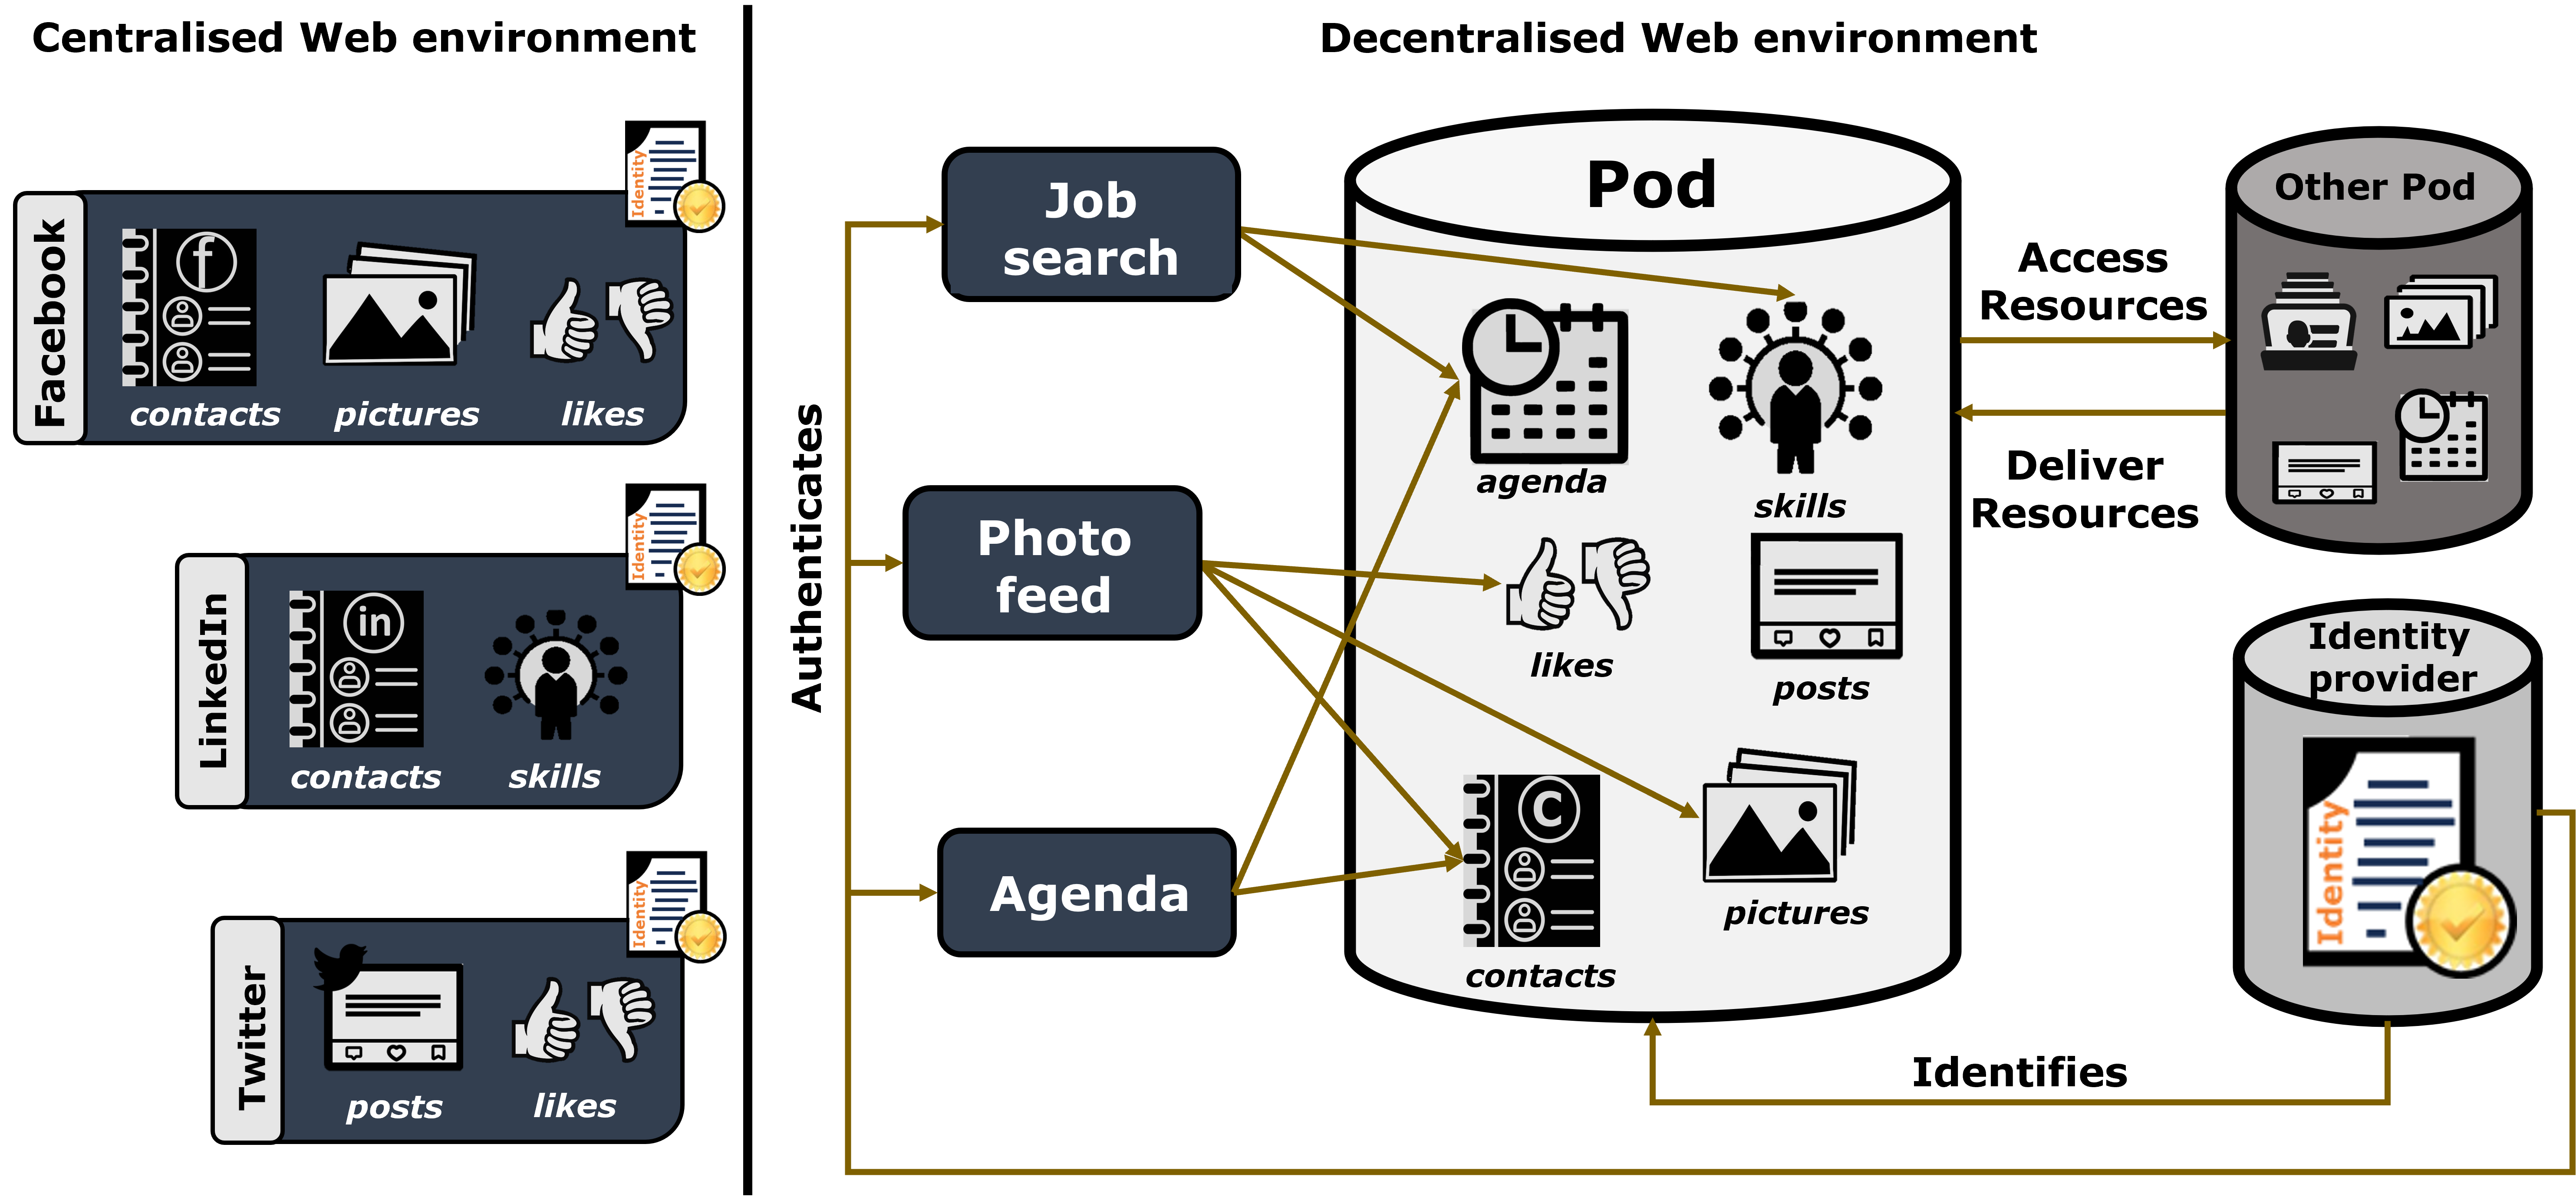
\includegraphics[width=\linewidth]{figures/chapter-1/decentralisation.png}
    \caption{Distinction between centralised and decentralised data environments.}
    \label{fig:decentralisation}
\end{figure}

% In this Thesis, we focus on providing users with the tools to better determine access to personal data resources stored in decentralised settings, according to EU law on personal data protection.
This Thesis focuses on providing users with the tools to better determine access to personal data resources stored in decentralised settings, according to EU law on personal data protection.
Beyond access control (\ref{sec:def_access_control}), usage control solutions also need to be developed to provide data subjects with \textit{``control over data usage once access to the data has been granted''}~\citep{akaichi_semantic_2022}.

\subsubsection{Personal datastores}
\label{sec:def_pds}

In its \textit{TechDispatch \#3/2020}~\citep{european_data_protection_supervisor_techdispatch_2021}, the EDPS envisioned the development of personal data spaces, managed through Personal Information Management Systems (PIMS) as a mechanism to enable personal data sovereignty where \textit{``Individuals, service providers and applications would need to authenticate to access a personal storage centre''} and individuals are able to \textit{``customize what categories of data they want to share and with whom''} while keeping a record of \textit{``who has had access to their digital behaviour''} and enabling data portability and interoperability.

Such decentralised systems (\ref{sec:def_decentralised_env}) allow data subjects to directly determine who has access to their data, and under which conditions, and can actually play an important role in facilitating the exercise of data subjects’ rights, including the rights of access, erasure, and data portability or the right to withdraw consent~\citep{janssen_personal_2020}.
In the last few years, different personal datastores initiatives have been gaining prominence and adoption, including the Solid project\footnote{\url{https://solidproject.org/} (accessed on 15 March 2024)}~\citep{fallatah_personal_2023}, which is the adopted use case for the research in this Thesis.

Solid is a free, open-source initiative that delivers on the promise of decentralising the storage of data by relying on Web standards and on Semantic Web vocabularies to promote data and services interoperability. To fulfil this vision, the Solid specification relies on authentication and authorisation protocols to provide private, secure, and granular access to data stored in Solid's personal online datastores, the so-called `Pods'~\citep{mansour_demonstration_2016}.